\documentclass[12pt]{article}

%%%%%%%%%%%%%%%%%%%%%%%%%%%%%%%%%%%%%%%%%%%%%%%%%%%%%%%%%%%%%%%%%%%%%%%%%%%%%%%%%%%%%%%%%%%%%%%%%%%%
% Math
\usepackage{fancyhdr} 
\usepackage{amsfonts}
\usepackage{amsmath}
\usepackage{amssymb}
\usepackage{amsthm}
%\usepackage{dsfont}

%%%%%%%%%%%%%%%%%%%%%%%%%%%%%%%%%%%%%%%%%%%%%%%%%%%%%%%%%%%%%%%%%%%%%%%%%%%%%%%%%%%%%%%%%%%%%%%%%%%%
% Macros
\usepackage{calc}

%%%%%%%%%%%%%%%%%%%%%%%%%%%%%%%%%%%%%%%%%%%%%%%%%%%%%%%%%%%%%%%%%%%%%%%%%%%%%%%%%%%%%%%%%%%%%%%%%%%%
% Commands and Custom Variables	
\newcommand{\problem}[1]{\hspace{-4 ex} \large \textbf{Problem #1} }
%\let\oldemptyset\emptyset
%\let\emptyset\varnothing
\newcommand{\norm}[1]{\left\lVert#1\right\rVert}
\newcommand{\sint}{\text{s}\kern-5pt\int}
\newcommand{\powerset}{\mathcal{P}}
\renewenvironment{proof}{\hspace{-4 ex} \emph{Proof}:}{\qed}
\newcommand{\solution}{\textit{Solution}:\bigbreak}
\newcommand{\RR}{\mathbb{R}}
\newcommand{\NN}{\mathbb{N}}
\newcommand{\QQ}{\mathbb{Q}}
\newcommand{\ZZ}{\mathbb{Z}}
\newcommand{\CC}{\mathbb{C}}
\newcommand{\VV}{\mathbb{V}}
\newcommand{\FF}{\mathbb{F}}
\renewcommand{\Re}{\operatorname{Re}}
\renewcommand{\Im}{\operatorname{Im}}

\newcommand{\bigO}{\mathcal{O}}

\renewcommand{\vec}[1]{\boldsymbol{\mathbf{#1}}}

\newcommand{\editnote}[1]{\textcolor{red}{\textbf{\MakeUppercase{#1}}}}


%%%%%%%%%%%%%%%%%%%%%%%%%%%%%%%%%%%%%%%%%%%%%%%%%%%%%%%%%%%%%%%%%%%%%%%%%%%%%%%%%%%%%%%%%%%%%%%%%%%%
%page
\usepackage[margin=1in]{geometry}
\usepackage{setspace}
%\doublespacing
\allowdisplaybreaks
\pagestyle{fancy}
\fancyhf{}
\rhead{Shaw \space \thepage}
\setlength\parindent{0pt}
\usepackage{color}

%%%%%%%%%%%%%%%%%%%%%%%%%%%%%%%%%%%%%%%%%%%%%%%%%%%%%%%%%%%%%%%%%%%%%%%%%%%%%%%%%%%%%%%%%%%%%%%%%%%%
%Code
\usepackage{listings}
\usepackage{courier}
\lstset{
	language=Python,
	showstringspaces=false,
	formfeed=newpage,
	tabsize=4,
	commentstyle=\itshape,
	basicstyle=\ttfamily,
}

%%%%%%%%%%%%%%%%%%%%%%%%%%%%%%%%%%%%%%%%%%%%%%%%%%%%%%%%%%%%%%%%%%%%%%%%%%%%%%%%%%%%%%%%%%%%%%%%%%%%
%Images
\usepackage{graphicx}
\graphicspath{ {images/} }
\usepackage{float}

%tikz
\usepackage[utf8]{inputenc}
%\usepackage{pgfplots}
%\usepgfplotslibrary{groupplots}

%%%%%%%%%%%%%%%%%%%%%%%%%%%%%%%%%%%%%%%%%%%%%%%%%%%%%%%%%%%%%%%%%%%%%%%%%%%%%%%%%%%%%%%%%%%%%%%%%%%%
%Hyperlinks
%\usepackage{hyperref}
%\hypersetup{
%	colorlinks=true,
%	linkcolor=blue,
%	filecolor=magenta,      
%	urlcolor=cyan,
%}

\begin{document}
	\thispagestyle{empty}
	
	\begin{flushright}
		Sage Shaw \\
		m567 - Fall 2018 \\
		\today
	\end{flushright}
	
\begin{center}{\large \textbf{Homework 3}}\end{center}
\bigbreak

%%%%%%%%%%%%%%%%%%%%%%%%%%%%%%%%%%%%%%%%%%%%%%%%%%%%%%%%%%%%%%%%%%%%%%%%%%%%%%%%%%%%%%%%%%%%%%%%%%%%
\hspace{-.5 ex}\problem{1(a)} For the two point boundary value problem
$$
u'' = p(x)u' + q(x)u + r(x), \ x \in [a,b], \ u(a)=\alpha, u(b)=\beta
$$
the function \texttt{fd2tpbvp} we discretize using using $m$ equally spaced points on the interior ($m+2$ total points) and solve using the second order finite difference approximations to the first and second derivatives.
\bigbreak

\begin{lstlisting}[language=python]
def fd2tpbvp(a,b,aplha,beta,p_func,q_func,r_func,m):
	h = (b-a)/(m+1)
	xs = np.linspace(a, b, m+2, endpoint=True)
	inner_xs = xs[1:-1]
	D2 = 1/h**2 * sp.diags([ [-2]*m, [1]*(m-1), [1]*(m-1) ],
			offsets=[0,1,-1], format='csr')
	D1 = 1/(2*h) * sp.diags([ [1]*(m-1), [-1]*(m-1) ], 
			offsets=[1,-1], format='csr')
	P = sp.diags(p_func(inner_xs))
	Q = sp.diags(q_func(inner_xs))
	r = r_func(inner_xs)
	
	A = D2-P@D1-Q
	rhs = r
	rhs[0] -= alpha/h*(1/h + p_func(a)/2)
	rhs[-1] -= beta/h*(1/h - p_func(b)/2)
	
	u = spla.spsolve(A, rhs)
	return np.block([alpha, u, beta]), xs
\end{lstlisting}
\bigbreak

%%%%%%%%%%%%%%%%%%%%%%%%%%%%%%%%%%%%%%%%%%%%%%%%%%%%%%%%%%%%%%%%%%%%%%%%%%%%%%%%%%%%%%%%%%%%%%%%%%%%
\problem{1(b)} For the particular problem
$$
u'' = 2\tan(x)u' + 2, \ x \in [0,1], \ u(0)=0, u(1)=0
$$
which has an exact solution of $u(x) = (x-1)\tan(x)$ we used the above function to solve it for $m= 10, 20, 40, 80, 160$. The results are seen in the plot below, and confirm that the method is $\mathcal{O}(h^2)$ accurate.

\begin{figure}[H]
	%\caption{Equispaced points}
	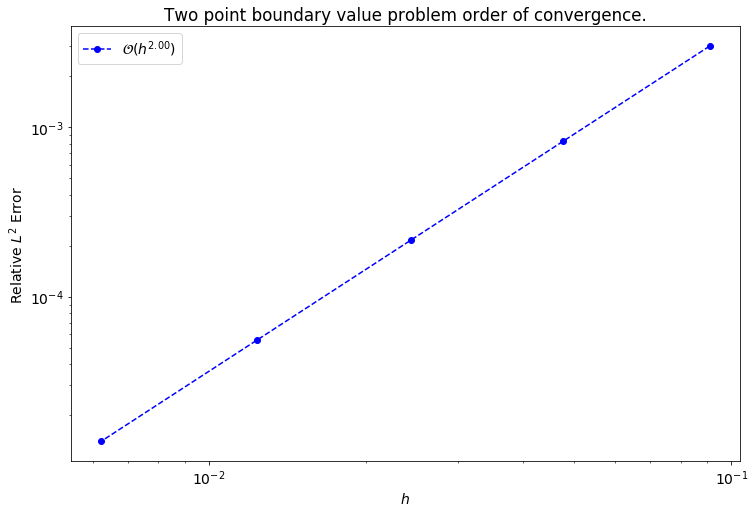
\includegraphics[width=1\textwidth]{hw03_p1b_order}
	\centering
\end{figure}
\bigbreak

%%%%%%%%%%%%%%%%%%%%%%%%%%%%%%%%%%%%%%%%%%%%%%%%%%%%%%%%%%%%%%%%%%%%%%%%%%%%%%%%%%%%%%%%%%%%%%%%%%%%
\problem{2(a)} For this problem I converted the MATLAB code in \texttt{chebdiffmat.m} to python3+Numpy in \texttt{cheb\_diff\_mat.py}.

\begin{lstlisting}
def cheb_diff_mat(n, m, a, b):
	thetas = np.linspace(0, np.pi, n, endpoint=True)
	T = np.repeat(.5*thetas.reshape((n,1)), n, axis=1)
	DX = 2 * np.sin(T.T + T) * np.sin(T.T - T)
	DX[n//2:] = -np.rot90(DX[:(n+1)//2], 2)
	DX[np.diag_indices(n)] = np.ones(n)
	C = (-1.0) ** np.add.outer(np.arange(n), np.arange(n))
	C[0]    *= 2
	C[-1]   *= 2
	C[:,0]  *= .5
	C[:,-1] *= .5
	Z = 1/DX
	Z[np.diag_indices(n)] = np.zeros(n)
	D = np.eye(n)
	DM = np.zeros((m,n,n))
	scale_factor = 1
	for i in range(m):
		D = (i+1)*Z*(C * np.multiply.outer(np.diag(D), 
							np.ones(n)) - D)
		D[np.diag_indices(n)] = -D @ np.ones(n)
		scale_factor *= 2/(b-a)
		DM[i] = scale_factor * D[::-1,::-1] 
				#account for flipping the points
	xs = -np.cos(thetas) #standard Chebyshev points
	xs = (xs+1) * (b-a)/2 + a #shifted
	return xs, DM
\end{lstlisting}

\bigbreak
%%%%%%%%%%%%%%%%%%%%%%%%%%%%%%%%%%%%%%%%%%%%%%%%%%%%%%%%%%%%%%%%%%%%%%%%%%%%%%%%%%%%%%%%%%%%%%%%%%%%
\problem{2(b)}
The code below uses this function to solve
$$
u'' = 2\tan(x)u' + 2, \ x \in [0,1], \ u(0)=0, u(1)=0
$$
for $m = 5, 10, 15, 20, 25, 30$.
\bigbreak

\begin{lstlisting}
def pstpbvp(a, b, p_func, q_func, r_func, m):
	alpha, beta = 0, 0
	h = (b-a)/(m+1)
	xs, D = cheb_diff_mat(m+2, 2, a, b)
	xs_all = xs
	xs = xs[1:-1]
	D_old = D
	D = D[:,1:-1,1:-1]
	P = sp.diags(p_func(xs))
	Q = sp.diags(q_func(xs))
	rhs = r_func(xs)
	A = D[1]-P@D[0]-Q
	u = la.solve(A, rhs)
	return u, xs
\end{lstlisting}

The errors can be seen in the plot below. Note that the order of convergence is quite large, as we would expect with a pseudo spectral method. This method converges far faster than the FD2 method and gives us the solution on the chebyshev points, which is ideal for interpolating to all points on our domain.

\begin{figure}[H]
	%\caption{Equispaced points}
	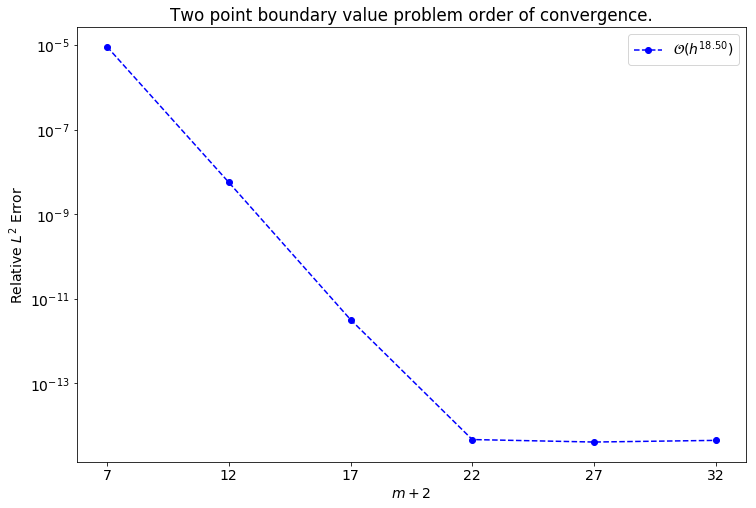
\includegraphics[width=1\textwidth]{hw03_p2b_pseudospectral}
	\centering
\end{figure}
\bigbreak

%%%%%%%%%%%%%%%%%%%%%%%%%%%%%%%%%%%%%%%%%%%%%%%%%%%%%%%%%%%%%%%%%%%%%%%%%%%%%%%%%%%%%%%%%%%%%%%%%%%%
\problem{3} In class we derived the discrete solution
$$
D_2\vec{u} - P D_1 \vec{u} - Q \vec{u} = \vec{r}
$$
which does not account for the boundary conditions. Here we will derive the formula that accounts for the right boundary condition $\beta_1 u(b) + \beta_2 u'(b) = \beta_3$. \bigbreak

After discretizing and using the fictitious point method we have $\beta_1 u_{m+1} + \beta_2u'_{m+1} = \beta_3$ or equivalently
$$
u'_{m+1} = \frac{\beta_3}{\beta_2} - \frac{\beta_1}{\beta_2}u_{m+1}.
$$
Using the second order approximation to the first derivative we have
\begin{align*}
	u'_{m+1} &= \frac{\beta_3}{\beta_2} - \frac{\beta_1}{\beta_2}u_{m+1} \\
	\frac{1}{2h}(-u_m + u_{m+2}) &= \frac{\beta_3}{\beta_2} - \frac{\beta_1}{\beta_2}u_{m+1} \\
	u_{m+2} &= 2h \left ( \frac{\beta_3}{\beta_2} - \frac{\beta_1}{\beta_2}u_{m+1} \right) + u_m.
\end{align*}

The last equation from our matrix system can be written as
\begin{align*}
\frac{1}{h^2}(u_m -2u_{m+1} + u_{m+2}) - p_{m+1}\frac{1}{2h}(u_{m+2} - u_m) - q_{m+1}u_{m+1} &= r_{m+1} \\
-u_m +2u_{m+1} - u_{m+2} + p_{m+1}\frac{h}{2}(u_{m+2} - u_m) + h^2q_{m+1}u_{m+1} &= -h^2r_{m+1} \\
-u_m + (2 + h^2q_{m+1})u_{m+1} - u_{m+2} + p_{m+1}\frac{h}{2}(u_{m+2} - u_m) &= -h^2r_{m+1} \\
-u_m + (2 + h^2q_{m+1})u_{m+1} - \left[ 2h \left ( \frac{\beta_3}{\beta_2} - \frac{\beta_1}{\beta_2}u_{m+1} \right) + u_m \right] + \phantom{===}&\\  p_{m+1}\frac{h}{2} \left[ 2h \left ( \frac{\beta_3}{\beta_2} - \frac{\beta_1}{\beta_2}u_{m+1} \right) + u_m - u_m \right] &= -h^2r_{m+1} \\
-2u_m + (2 + h^2q_{m+1})u_{m+1} + 2h \left ( -\frac{\beta_3}{\beta_2} + \frac{\beta_1}{\beta_2}u_{m+1} \right) + \phantom{===}&\\ p_{m+1}h^2 \left ( \frac{\beta_3}{\beta_2} - \frac{\beta_1}{\beta_2}u_{m+1} \right) &= -h^2r_{m+1} \\
-2u_m + \left( 2 + h^2q_{m+1} + 2h\frac{\beta_1}{\beta_2}  - p_{m+1}h^2 \frac{\beta_1}{\beta_2} \right) u_{m+1} &= \\ -h^2r_{m+1} + 2h\frac{\beta_3}{\beta_2} &- ph^2 \frac{\beta_3}{\beta_2} \\
-2u_m + \left[ 2 + h^2q_{m+1} + (2 - hp_{m+1}) h\frac{\beta_1}{\beta_2} \right] u_{m+1} = -h^2r_{m+1} &+ (2 - hp_{m+1}) h \frac{\beta_3}{\beta_2}
\end{align*}
which is the desired formula.

\bigbreak
%%%%%%%%%%%%%%%%%%%%%%%%%%%%%%%%%%%%%%%%%%%%%%%%%%%%%%%%%%%%%%%%%%%%%%%%%%%%%%%%%%%%%%%%%%%%%%%%%%%%
\problem{4(a)} Show that the linear system (5) has a unique solution regardless of $\vec{b}$. \bigbreak

\begin{proof}
	If we let the right hand side be the zero vector, and show that $\vec{u}=\vec{0}$ and $\lambda=0$, we will have shown that the matrix is one-to-one. Any linear operator on a finite-dimensional vector space is invertible (ie. has a unique solution) if it is one-to-one. \bigbreak
	
	Let (i) $A\vec{u} + \lambda \vec{w} = \vec{0}$ and let (ii) $\vec{w}^T\vec{u} = 0$. \bigbreak
	
	Multiply (i) on the left by $\vec{w}^T$ and note that $\vec{w}^TA = \vec{0}$. This is clear since $\frac{1}{2}(-2) + 1*1 = 0$ and $\frac{1}{2}(2) - 1*2 + 1*1=0 $. The first equation shows that the first and last elements of the vector are zero, while the second shows that all interior points of the vector are zero. Thus we have $\vec{w}^TA = \vec{0}$ and $\vec{w}^T \lambda =\vec{0}$. Clearly $\lambda = 0$. \bigbreak
	
	Now we have that $A\vec{u} = \vec{0}$. The first equation in this system shows us that $u_0 = u_1$. The second shows that $u_2 = u_0$. Continuing to the last row we get that $u_0 = u_1 = u_2 = \dots = u_{m+1} = \alpha$ for some constant $\alpha$. Then $0 = \vec{w}^T\vec{u} = \alpha(m+0.5)$ and thus $\vec{u} = \vec{0}$. \bigbreak
	
	This shows that the system is always one-to-one and thus invertible, and thus will always have a unique solution regardless of $\vec{b}$.
\end{proof}

\bigbreak
%%%%%%%%%%%%%%%%%%%%%%%%%%%%%%%%%%%%%%%%%%%%%%%%%%%%%%%%%%%%%%%%%%%%%%%%%%%%%%%%%%%%%%%%%%%%%%%%%%%%
\problem{4(b)} Show that if $\vec{w}^T\vec{b} = 0$ then $\lambda = 0$. This shows that the solution $\vec{u}$ will approximately solve the original differential equation. \bigbreak

\begin{proof}
	From above we have that
	\begin{align*}
		A\vec{u} + \lambda \vec{w}&= \vec{b} \\
		\vec{w}^T A\vec{u} + \lambda \vec{w}^T \vec{w} &= \vec{w}^T \vec{b} \\
		\lambda \vec{w}^T \vec{w} &= \vec{w}^T \vec{b} \\
		\lambda (m+0.5) &= \vec{w}^T \vec{b} \\
		\lambda &= \frac{1}{m+0.5} \vec{w}^T \vec{b}
	\end{align*}
	Thus $\vec{w}^T \vec{b} = 0 \implies \lambda=0$.
\end{proof}

\bigbreak
%%%%%%%%%%%%%%%%%%%%%%%%%%%%%%%%%%%%%%%%%%%%%%%%%%%%%%%%%%%%%%%%%%%%%%%%%%%%%%%%%%%%%%%%%%%%%%%%%%%%
\problem{4(c)} Here we solve the 1D Poisson equation with Neumann boundary conditions:
$$
u''(x) = -4\cos(2x), \ 0 \leq x \leq 2\pi, \ u'(0)=u'(2\pi)=0
$$
by using the DF2 approximations to the second derivative at $m=99$ interior points on the domain, and the method of Lagrange multipliers enforcing the condition that the total mass of the system is zero.
\begin{lstlisting}
m = 99
a, b, = 0, 2*np.pi
sa, sb = 0, 0
sa, sb = -np.pi**2, np.pi**2
U = 0 #(sb-sa)/(b-a)
def foo(x):
	return -4*np.cos(2*x)
xs = np.linspace(a, b, m+2, endpoint=True)
h = (b-a)/(m+1)
A  = np.diag([-2.0]*(m+2))
A += np.diag([1]*(m+1), k=1)
A += np.diag([1]*(m+1), k=-1)
A[0,1] = 2
A[-1,-2] = 2
A *= h**-2
fs = foo(xs)
fs[0]  += 2/h * sa
fs[-1] -= 2/h * sb
w = np.ones(m+2)
w[0] = .5
w[-1] = .5
M = np.block([[A, w.reshape((m+2,1))],[w, 0]])
rhs = np.zeros(m+3)
rhs[:-1] = foo(xs)
rhs[-1] = U*(m+1)
us = la.solve(M, rhs)
lam = us[-1]
us = us[:-1]
\end{lstlisting}
\bigbreak

When executed we get a value for $\lambda$ that is zero to machine precision and a relative $L^2$ error of $\approx 0.00131699$. The vector approximating the solution can be seen in the plot below.

\begin{figure}[H]
	%\caption{Equispaced points}
	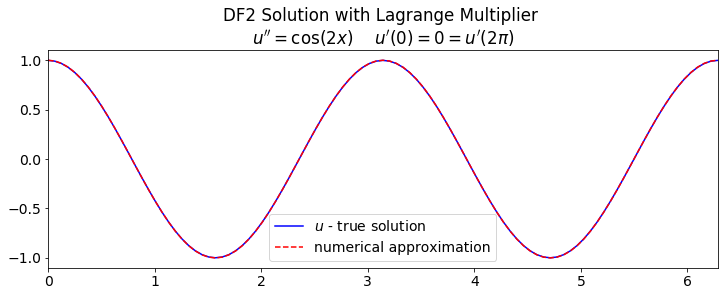
\includegraphics[width=1\textwidth]{hw03_p4c}
	\centering
\end{figure}
\begin{figure}[H]
	%\caption{Equispaced points}
	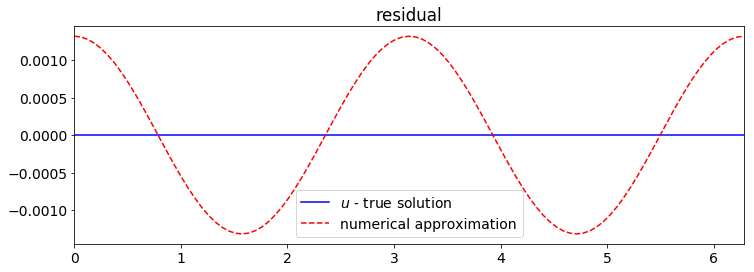
\includegraphics[width=1\textwidth]{hw03_p4c_residual}
	\centering
\end{figure}

\bigbreak
%%%%%%%%%%%%%%%%%%%%%%%%%%%%%%%%%%%%%%%%%%%%%%%%%%%%%%%%%%%%%%%%%%%%%%%%%%%%%%%%%%%%%%%%%%%%%%%%%%%%
\problem{4(d)} Consider the problem
\begin{align}
u''(x) = x, \ 0 \leq x \leq 2\pi, \ u'(0)=-\pi^2, \ u'(2\pi)=\pi^2 \label{original_ode}
\end{align}
which is has non-homogeneous boundary conditions. Since $\int_0^{2\pi}x dx = 2\pi^2 = u'(2\pi)-u'(0)$ this problem satisfies the continuous compatibility condition and thus has a unique solution up to a constant. 
\bigbreak

It is easy to see that $u(x) = \frac{1}{6}x^3 - \pi^2x + C$ satisfies this equation.
Adding the additional arbitrary criteria that the total mass is zero $\int_0^{2\pi} u(x) dx = 0$ we get
$$
u(x) = \frac{1}{6}x^3 - \pi^2x + \frac{2\pi^3}{3}
$$
as a true solution. When we run the algorithm we get $\lambda$ is zero to machine precision, and a relative $L^2$ error of $\approx 0.000183756$. The value $\lambda$ tells us how close we are to satisfying the differential equation. Since $\lambda$ is essentially zero, we can say that our solution satisfies the differential equation and our approximation is a good estimate to the solution.

\begin{figure}[H]
	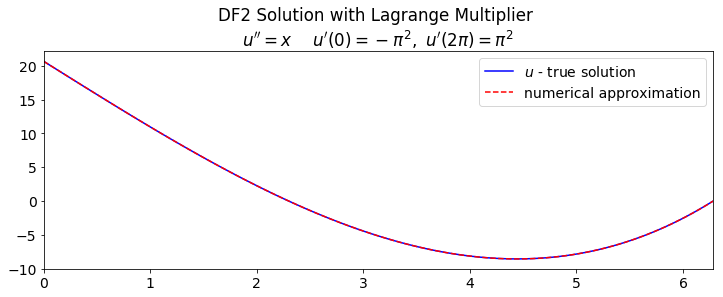
\includegraphics[width=1\textwidth]{hw03_p4d}
	\centering
\end{figure}
\begin{figure}[H]
	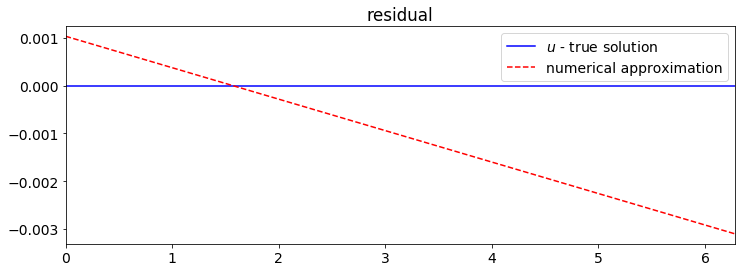
\includegraphics[width=1\textwidth]{hw03_p4d_residual}
	\centering
\end{figure}

\bigbreak
%%%%%%%%%%%%%%%%%%%%%%%%%%%%%%%%%%%%%%%%%%%%%%%%%%%%%%%%%%%%%%%%%%%%%%%%%%%%%%%%%%%%%%%%%%%%%%%%%%%%
\problem{4 Conclusion} In both of the examples above the compatibility condition was met and the solution we found approximated the true solution with the zero total mass criteria. I was curious what a non-zero value of $\lambda$ would mean so I tested the following similar example:
\begin{align}
u''(x) = x, \ 0 \leq x \leq 2\pi, \ u'(0)=0, \ u'(2\pi)=0.
\end{align}
This example does not meet the compatibility condition. When computed it gives a value of $\lambda$ of roughly $\pi$.  This tells me that $A\vec{u} + \lambda \vec{w} \approx \vec{f}$ in the discrete case and would suggest that $u''(x) - \lambda = x$. Or in particular, that our approximate solution solves the differential equation
\begin{align}
u''(x) = x-\pi, \ 0 \leq x \leq 2\pi, \ u'(0)=0, \ u'(2\pi)=0.
\end{align}
which \textit{does} satisfy the compatibility condition and has a true solution of 
$$
u(x) = \frac{1}{6}x^3 - \frac{\pi}{2}x^2 + \frac{\pi^3}{3}.
$$
This is confirmed in the plot below and gives a relative $L^2$ error of $\approx 0.00327647$.

%When we run our algorithm with these parameters we get $\lambda = 3.15738 \approx \pi$. The result can be seen in the plot below.
%
%\begin{figure}[H]
%	%\caption{Equispaced points}
%	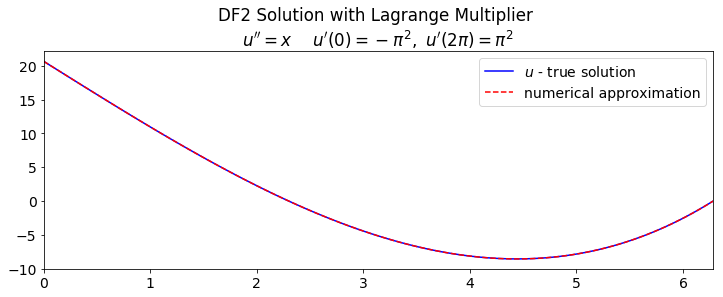
\includegraphics[width=1\textwidth]{hw03_p4d}
%	\centering
%\end{figure}
%
%Clearly this is a terrible approximation to the solution of the differential equation, but it was not in vain. Notice that our result is nearly flat at the boundaries. In light of this, consider modified differential equation with homogeneous Neumann boundary conditions:
%$$
%u_{a}''(x) = x - \lambda, \ 0 \leq x \leq 2\pi, \ u_{a}'(0)=0=u_{a}'(2\pi).
%$$
%Here we choose $\lambda$ such that we satisfy the continuous compatibility condition $\int_0^{2\pi}x-\lambda dx = 0$ which results in $\lambda = \pi$. When we integrate twice we see that $u_{h}(x) = \frac{1}{6}x^3 - \frac{\pi^2}{2}x^2 + C$. Specifying that the total mass be zero $\int_0^{2\pi}u_{a}(x) dx = 0$ we get the solution
%$$
%u_{a}(x) = \frac{1}{6}x^3 - \frac{\pi^2}{2}x^2 + \frac{\pi^3}{3}.
%$$
%\bigbreak
%
%Next we consider a similar almost-homogeneous differential equation:
%$$
%u_{h}''(x) = \lambda, \ 0 \leq x \leq 2\pi, \ u_{h}'(0)=-\pi^2, \ u_{h}'(2\pi)=\pi^2.
%$$
%Again integrating twice we have that $u_h(x) = \frac{\pi}{2}x^2 - \pi^2 x + C$, and requiring the total mass to be zero: $\int_0^{2\pi}u_h(x)dx = 0$ we arrive at the solution
%$$
%u_{h}(x) = \frac{\pi}{2}x^2 - \pi^2 x + \frac{\pi^3}{3}.
%$$
%\bigbreak
%
%The solution $u_a$ is the solution that our discrete method is approximating. By superposition, the sum $u_a + u_h$ is a solution to the original differential equation (\ref{original_ode}). The plot below, shows that our solution approximates $u_a$, and when summed with $u_h$ approximates our true solution.




\bigbreak
%%%%%%%%%%%%%%%%%%%%%%%%%%%%%%%%%%%%%%%%%%%%%%%%%%%%%%%%%%%%%%%%%%%%%%%%%%%%%%%%%%%%%%%%%%%%%%%%%%%%
\problem{5(a)} Substituting our IDCT expressions for $u_j$ into our linear system yields
\begin{align*}
	\left(h^2A\vec{u} \right)_j = u_{j-1} -2u_j + u_{j+1} &= 2 \sum\limits_{k=0}^{m+1}{}^{''} \hat{u}_k \left[  \cos\left( \frac{\pi k (j-1)}{m+1} \right) \right. \\
	&\phantom{===}\left. - 2 \cos\left( \frac{\pi k j}{m+1} \right) + \cos\left( \frac{\pi k (j+1)}{m+1} \right) \right].
\end{align*}
Recall the trigonometric identity $\cos \alpha + \cos \beta = 2 \cos\frac{\alpha +\beta}{2}\cos\frac{\alpha -\beta}{2}$ and apply it to the terms $\cos\left( \frac{\pi k (j-1)}{m+1} \right) + \cos\left( \frac{\pi k (j+1)}{m+1} \right)$ to get 
$$
\cos\left( \frac{\pi k (j-1)}{m+1} \right) + \cos\left( \frac{\pi k (j+1)}{m+1} \right) = 2\cos\left( \frac{\pi k j}{m+1} \right)\cos\left( \frac{\pi k}{m+1} \right)
$$
Thus we have that the left-hand side is 
\begin{align*}
	\left(h^2A\vec{u} \right)_j & = 2  \sum\limits_{k=0}^{m+1}{}^{''} \hat{u}_k \left[  \cos\left( \frac{\pi k (j-1)}{m+1} \right) - 2 \cos\left( \frac{\pi k j}{m+1} \right) + \cos\left( \frac{\pi k (j+1)}{m+1} \right) \right] \\
	&= 2  \sum\limits_{k=0}^{m+1}{}^{''} \hat{u}_k \left[  2\cos\left( \frac{\pi k j}{m+1} \right) 2\cos\left( \frac{\pi k}{m+1} \right) - 2 \cos\left( \frac{\pi k j}{m+1} \right)  \right] \\
	&= 2  \sum\limits_{k=0}^{m+1}{}^{''} \hat{u}_k \left[  2\cos\left( \frac{\pi k}{m+1} \right) - 2 \right] \cos\left( \frac{\pi k j}{m+1} \right) .
\end{align*}

The right-hand side is simply $h^2f = h^2 2 \sum\limits_{k=0}^{m+1}{}^{''} \hat{f}_k\cos\left( \frac{\pi k j}{m+1} \right)$. Dividing each side by $2$, and equating them we have
$$
\sum\limits_{k=0}^{m+1}{}^{''} \hat{u}_k \left[  2\cos\left( \frac{\pi k}{m+1} \right) - 2 \right] \cos\left( \frac{\pi k j}{m+1} \right) =  \sum\limits_{k=0}^{m+1}{}^{''} h^2\hat{f}_k\cos\left( \frac{\pi k j}{m+1} \right)
$$
as desired. The cases of $j=0$ and $j= m+1$ appear slightly different, our two equations corresponding to those points are algebraically equivalent to the same equation applied to the three point stencils centered at the endpoints and including our fictitious points. Thus the result is the same.

\bigbreak
%%%%%%%%%%%%%%%%%%%%%%%%%%%%%%%%%%%%%%%%%%%%%%%%%%%%%%%%%%%%%%%%%%%%%%%%%%%%%%%%%%%%%%%%%%%%%%%%%%%%
\problem{5(b)} With regard to the result above, recall that the IDCT is the inverse of the DCT we have that 
\begin{align*}
	\hat{u}_k \left( 2 \cos \left(\frac{\pi k}{m+1} \right) - 2 \right) &= h^2\hat{f}_k \\
	\hat{u}_k &= \frac{h^2\hat{f}_k}{2 \cos \left(\frac{\pi k}{m+1} \right) - 2}
\end{align*}
\bigbreak

Show how $\hat{f}_0 = 0$ is analogous to the discrete compatibility condition $\vec{w}^T\vec{b} = \vec{w}^T\vec{f} = 0$.  \bigbreak

By definition $\hat{f}_0 = \frac{1}{m+1}\sum\limits_{j=0}^{m+1} {}^{\prime\prime} f_j \approx \int_{a}^{b} f(x) dx$ which is the compatibility condition.

\bigbreak
%%%%%%%%%%%%%%%%%%%%%%%%%%%%%%%%%%%%%%%%%%%%%%%%%%%%%%%%%%%%%%%%%%%%%%%%%%%%%%%%%%%%%%%%%%%%%%%%%%%%
\problem{5(c)} Given a forcing function $u''(x) = f(x)$, we discretize in the usual way so that there are $m+2$ total equally spaced points on the interval $[a, b]$ and approximate the function $f$ with the vector $\vec{f}$. We then calculate $\hat{\vec{f}}$ and use the formula in part (b) to calculate $\hat{\vec{u}}$. That is except for the first entry $\hat{u}_0$. For this entry we set $\hat{u}_0 = U$ for some arbitrary choice of $U$. Since $\hat{u}_0 = \sum\limits_{j=0}^{m+1}{}^{\prime\prime} u_j \approx \int_a^{b} u(x) dx$ we can think of $U$ as the total mass of the solution. \bigbreak

After setting $\hat{u}_0$ we compute $\vec{u}$ via the IDCT and we have our approximate solution.

\bigbreak
%%%%%%%%%%%%%%%%%%%%%%%%%%%%%%%%%%%%%%%%%%%%%%%%%%%%%%%%%%%%%%%%%%%%%%%%%%%%%%%%%%%%%%%%%%%%%%%%%%%%
\problem{5(d)} The following code solves the problem in 4(c) using the DCT to solve the system. Setting $\hat{f}_0 = 0$ is the discrete version of the zero-total-mass criterion.

\begin{lstlisting}
m = 10**4
h = (b-a)/(m+1)
xs = np.linspace(a, b, m+2, endpoint=True)
fs = foo(xs)

# fft.dct(xs, type=1)/(2*n-2)
# scipy needs to be scaled to match our form

f_hat = fft.dct(fs, type=1)/(2*m+2)
u_hat = np.zeros(len(xs))
u_hat[1:] = h**2 * f_hat[1:] / 
			(2*np.cos(np.pi*np.arange(1,m+2)/(m+1)) - 2)
u_hat[0] = 0 # arbitrary
us = fft.idct(u_hat)
\end{lstlisting}

When executed this algorithm gives a relative $L^2$ error of $\approx 0.00131699$, exactly the same as problem 4(c). The plot is shown below.

\begin{figure}[H]
	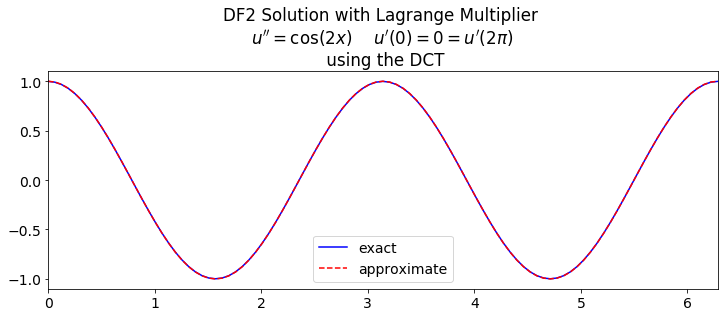
\includegraphics[width=1\textwidth]{hw03_p5d}
	\centering
\end{figure}
\begin{figure}[H]
	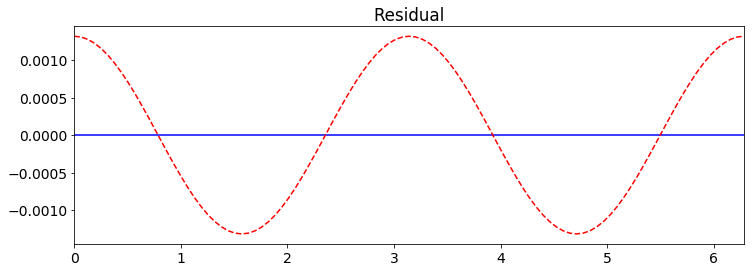
\includegraphics[width=1\textwidth]{hw03_p5d_residual}
	\centering
\end{figure}

\bigbreak
%%%%%%%%%%%%%%%%%%%%%%%%%%%%%%%%%%%%%%%%%%%%%%%%%%%%%%%%%%%%%%%%%%%%%%%%%%%%%%%%%%%%%%%%%%%%%%%%%%%%
\problem{5(e)} I'm not sure I understand what this is asking. I think that parts (a) and (b) prove that they are mathematically equivalent. In part (a) we substituted $A\vec{u} = A T_{\cos}^{-1}(\hat{\vec{u}})$ (and similarly for the right-hand side) where $T_{\cos}^{-1}$ denotes the inverse discrete cosine transform. These are mathematically equivalent. Since the DCT and IDCT are bijections we can equate their arguments as we did in part (b). The rest is a little algebra a trig identity and applying the IDCT again. \bigbreak

Of course numerically they will likely have different round-off error.
\end{document}
